\chapter{Testing and Results}\label{ch:results}

\section{Test Data}\label{se:res.testdata}
There are two data sets that I have tested the implementation with: (1) handwritten digits data set from~\cite{Ng12}; and, (2) handwritten digits data set from~\cite{LeCCorBur}.

Set (1) consists of $5000$ training examples of $20 \times 20$ pixel greyscale images of digits, each pixel represented by a floating point number that indicates the greyscale intensity at that location. The input layer will thus have 400 neurons. In this example, the hidden layer has 25 neurons and the output layer has 10 neurons. The size of weight vector between input and hidden layers is $401 \times 25 = 10025$ and the size of the weight vector between hidden and output layers is $26 \times 10 = 260$. 

The output neuron with the highest activation value will be the digit that the sample will be classifed under. For instance, if the neuron `4' of the output vector, \texttt{ys[3]} had the highest value, then the sample will be classified as digit `4'.

This data set was mostly used during the development to assess the accuracy of the implementation, as I could easily compare the values produced by my program with the values from the MATLAB program. In ~\ref{se:res.performance} I evaluated the comparative performance of Accelerate and MATLAB, up to 2 cores.

Set (2) is Le Cunn's MNIST handwritten digits database. This consists of a training set of $60000$ examples and a test set of $10000$ examples. Each example is a $28 \times 28$ pixel greyscale image. This input layer has 784 neurons and a hidden layer of 300 neurons. Thus the size of weight vector between them is $785 \times 300 = 235500$. The size of weight vector between hidden and output layer is $301 \times 10 = 3010$. This data set was used to test the performance of completed Accelerate implementation from 1 to 8 cores.

Each test was repeated 10 times and the average value plotted. The initial weight vectors for training set (2) benchmarking was kept consistent to strictly measure the effect of cores on performance. In training set (1), the initial weight are randomly initialised, and thus up to 1\% in fluctuations could result from this factor~\cite{Ng12}.
 
\section{Testing environment}\label{se:res.testsys}
There are two testing environments. Both environments ran on \texttt{llvm} backends as the testing data was too small for the GPU backend. 

The first configuration is for testing during development. It is a 2-core Intel i5-5200U CPU (64-bit, 2.2GHz, 12GB RAM, hyperthreading enabled) running GNU/Linux (Ubuntu 16.04 LTS). 

The second configuration was for dedicated multi-core testing. It is a 4-core "Ivy Bridge" Intel i7-3720QM (64-bit, 2.6GHz, 8GB SDRAM, hyperthreading enabled) running MacOS.

\section{Performance results}\label{se:res.performance}

Table \ref{tb:acc.vs.matlab} shows that in the development environment with training sample set (1), the accuracy of the Accelerate implementation is similar to MATLAB's; however, the time taken to calculate the weights grows much faster depending on the sample size. This may be due to some bugs mentioned in Chapter~\ref{ch:eval}.

\begin{table}
\centering
\resizebox{\textwidth}{!}{
	\begin{tabular}[width=\linewidth]{| r | p{3cm} | p{3cm} | p{3cm} | p{3cm} |}
    \hline
    Input size & Accelerate (LLVM-CPU)(s) & Accelerate accuracy (\%) & MATLAB (s) & MATLAB accuracy (\%) \\ \hline
     100 & 0.4912 	& 75.22 	& 0.2037 	& 75.00  \\ \hline
     250 & 0.9312	& 83.42 	& 0.3592 	& 83.84  \\ \hline
     500 & 1.545 	& 88.86 	& 0.5028 	& 88.66  \\ \hline
     750 & 2.106 	& 89.94 	& 0.7283 	& 89.94  \\ \hline
    1000 & 2.821 	& 91.40  	& 0.8276 	& 90.90  \\ \hline
    1500 & 4.052 	& 92.64 	& 1.2782 	& 92.40  \\ \hline
    2000 & 5.915 	& 93.44 	& 1.3827 	& 93.62  \\ \hline
    3000 & 8.273 	& 94.10 	& 1.9658 	& 94.50  \\ \hline
    4000 & 13.1 	& 94.74 	& 2.4011 	& 94.96  \\ \hline
    5000 & 17.95 	& 95.54 	& 2.6811 	& 95.08  \\ 
    \hline
	\end{tabular}}
	\caption{Benchmarking training set 1 (Training set from \cite{Ng12}).}
	\label{tb:acc.vs.matlab}
\end{table}

\begin{table}
\centering
\resizebox{\textwidth}{!}{
	\begin{tabular}[width=\linewidth]{| c | c | c |}
    \hline
    Number of cores & Accelerate (LLVM-CPU)(s) & Accelerate accuracy (\%) \\ \hline
     1 & 239.695	& 83.97 	\\ \hline
     2 & 184.37  	& 84.46 	\\ \hline
     3 & 151.967 	& 84.46 	\\ \hline
     4 & 135.719	& 84.46 	\\ \hline
     5 & 133.421	& 84.46  	\\ \hline
     6 & 130.372 	& 84.46 	\\ \hline
     7 & 124.314 	& 84.46 	\\ \hline
     8 & 122.310 	& 84.46 	\\ 
    \hline
	\end{tabular}}
	\caption{Benchmarking training set 2 (MNIST training set).}
	\label{tb:acc.vs.cores}
\end{table}

Table \ref{tb:acc.vs.cores} indicates a performance improvement with the addition of more cores. It levels off rapidly, however, perhaps indicating that there may be too much overhead to keep the cores synchronized to gain more benefit with the current implementation (see Chapter~\ref{ch:eval}).

Another alarming result is the lower than expected accuracy at 84.46\%. At \texttt{lambda=3.0}, this remains largely unchanged at 84.39\%. I checked the MATLAB accuracy with training set (2) and got an average of 91.68\% accuracy and 190.52 seconds time taken (10 tests on first testing environment), indicating that the issues outlined in~\ref{se:impl.limits} is having a significant impact on correctness of my implementation.

\begin{figure}
\centerline
	{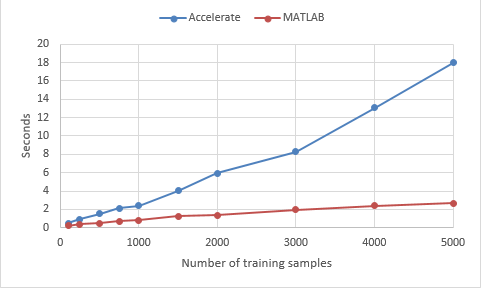
\includegraphics[scale=0.7]{training1.png}}
\centerline	
	{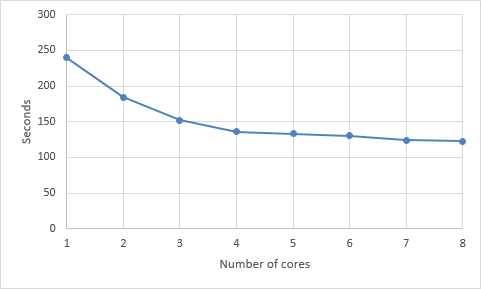
\includegraphics[scale=0.7]{training2.png}}
	\caption{Graphs of training set 1 (top) and 2 (bottom) benchmarks.}
	\label{fig:traininggraphs}
\end{figure}
